\documentclass{beamer}
\usepackage{amsmath,amssymb,amsthm,array}
\usepackage{xltxtra}
\usepackage{multirow}
\usepackage{multicol}
\usepackage{algorithm}
\usepackage{algorithmic}
\usetheme{CambridgeUS}
\usecolortheme{dolphin}
\usefonttheme{serif}
\setbeamertemplate{navigation symbols}{}
\title{Homomorphic Voting Schemes}
\author{Panagiotis Grontas}
\date{22/11/2013}
\setbeamertemplate{footline}
{
  \leavevmode%
  \hbox{%
  
  \begin{beamercolorbox}[wd=1\paperwidth,ht=2.25ex,dp=1ex,right]{title in head/foot}%
    \usebeamerfont{title in head/foot}\insertshorttitle\hspace*{3em}
    \insertframenumber{} / \inserttotalframenumber\hspace*{1ex}
  \end{beamercolorbox}}%
  \vskip0pt%
}
 
\institute{$\mu\Pi\lambda\forall$  - CoReLab Crypto Group}

\newcommand{\zns}[1]{ \mathbb{Z}_{#1}^* }
\newcommand{\zn}[1]{ \mathbb{Z}_{#1}}
\newcommand{\md}[1]{\quad (mod \, {#1})}

\setlength{\columnseprule}{0.4pt}
\begin{document}

\begin{frame}
\titlepage
\end{frame}

\begin{frame}{Introduction}
\begin{itemize}
\item Voting secrecy $\rightarrow$ Encrypt the votes
\item Calculate the result: Decrypt each vote and count
\item What if we could calculate the result without decrypting the votes;
\item Solution: Homomorphic Cryptosystems
\begin{itemize}
\item Encrypt votes under authority public key
\item Combine ciphertexts
\item $ E(v_1) \otimes \cdots \otimes E(v_n) = E(v_1 \oplus \cdots \oplus v_n) $
\item Result: Encrypted vote aggregate
\item Decrypt using the (shared) authority private key
\end{itemize}
\end{itemize}
\end{frame}

\begin{frame}{Homomorphic Cryptosystems}
\begin{block}{}
Ballot secrecy under cryptographic assumptions
\end{block}
\begin{itemize}
\item The RSA and the El Gamal cryptosystem is multiplicatively homomorphic.
	\begin{itemize}
		\item $ E(m_1)E(m_2) = m_{1}^{e} m_2^e \md{n} = (m_1 m_2)^e \md{n} = E(m_1 m_2) $
		\item $ E(m_1)E(m_2) = (g^{r_1},m_1 h^{r_1}) (g^{r_2},m_2 h^{r_2}) =  (g^{r_1+r_2}, m_1 m_2 h^{r_1+r_2}) = E(m_1 m_2)$
	\end{itemize}
\item The exponential El Gamal cryptosystem is additively homomorphic.
	\begin{itemize}
		\item $ E(m_1)E(m_2) = (g^{r_1},g^{m_1} h^{r_1}) (g^{r_2},g^{m_2} h^{r_2}) =  (g^{r_1+r_2}, g^{m_1 + m_2} h^{r_1+r_2}) = E(m_1 + m_2)$
	\end{itemize}
\item The Goldwasser Micali and the Benaloh Cryptosystems are additively homomorphic.
	\begin{itemize}
		\item $ E(m_1)E(m_2) =  y^{m_1} r_1^{2} y^{m_2} r_2^{2} = y^{m_1+m_2} (r_1r_2)^2 = E(m_1+m_2)$
		\item $ E(m_1)E(m_2) =  y^{m_1} x_1^{r} y^{m_2} x_2^{r} = y^{m_1+m_2} (x_1x_2)^r = E(m_1+m_2)$
	\end{itemize}
\item The Paillier cryptosystem is additively homomorphic.
	\begin{itemize}
		\item $ E(m_1)E(m_2) =  (1+n)^{m_1} r_1^{n^s} (1+n)^{m_2} r_2^{n^s} \md{n^{s+1}}= E(m_1 + m_2)$
	\end{itemize}
\end{itemize}
\end{frame}

\begin{frame}{The homomorphic secret sharing approach}
\begin{block}{}
Initial Aim: Ballot secrecy under no assumptions
\end{block}

\begin{itemize}
\item A \textit{super secret} $S$ can be computed from $m$ \textit{sub secrets} $\{ S_i \}_{i=1}^m$ $S = f(S_1,...,S_m)$
\item Each of the sub secret holder acts as the dealer in the secret sharing scheme and deals the shares into $n$ entities $ \{ E_j \}_{j=1}^n $ each receiving $ \{ S_{ij} \}_{i=1,j=1}^{m,n}$. 
\item Each entity combines its shares $R_j = g( S_{1j},...,S_{mj} )$ 
\item A subset of the entities reconstruct $S$ using the secret sharing scheme.
\end{itemize} 
\begin{tiny}
\begin{align*}
  S \leftarrow_{f}  
  \left[ \begin{array}{c} S_{1} \\ S_{2} \\ \cdots \\ S_{m} \end{array} \right]
  \rightarrow_{share} 
  \left[ \begin{array}{ccc} E_{1} &  \cdots & E_{n} \end{array} \right] 
  \rightarrow
  \left[ \begin{array}{ccc}  S_{11} & \cdots & S_{1n} \\ S_{21} & \cdots & S_{2n} \\ & \cdots & \\ S_{m1} & \cdots & S_{mn}   \end{array}  \right]
  \rightarrow
  \left[ \begin{array}{ccc}   g(S_{11}, \cdots, S_{1n}) \\ g(S_{21}, \cdots, S_{2n}) \\  \cdots  \\g(S_{m1}, \cdots, S_{mn})   \end{array} \right]
  \rightarrow
  S
\end{align*}
\end{tiny}
\end{frame}

\begin{frame}{The problem}
\begin{itemize}
\item Encryption promotes secrecy but hinders integrity, fairness
\item Attacks:
	\begin{itemize}
		\item Vote cancelling: Instead of encrypting a normal vote $v \in \{ 0,1 \}$, encrypt 1000 or -1000
		\item Authority aggregates extra votes or discards votes
		\item Refuse to decrypt the tally
	\end{itemize}
\item Solution: Add controls that increase
	\begin{itemize}
		\item Fairness
		\item Verifiability
		\item Robustness
	\end{itemize}
\end{itemize}
\end{frame}

\begin{frame}[allowframebreaks]{Benaloh Cryptosystem}
\begin{block}{$r-residues$}
$y$ is an $r-residue \quad \md{n}$ if $\exists x: y = x^r \md{n}$. 

Trapdoor: $n$ has known factorisation, it is easy to recognise an $r-residue$. 
\end{block}

\begin{itemize}
\item \textbf{Key Generation} 
\begin{itemize}
\item Agree on a prime number $r$ known to every participant.
\item Select randomly and independently two large primes $p,q$ such that $r \shortmid (p-1)$ and $r \nshortmid (q-1) $
\item Calculate the RSA modulus $n = p \cdot q$
\item Select a \textit{quadratic \textbf{non}-residue}. $y \in \zns{n}$ with $gcd(y,n)=1$. 
\item The public key is $N,y$
\item The private key is $p,q$
\end{itemize}
\item \textbf{Encryption}
\begin{itemize}
\item $c = E(m) = y^{m} x^r \md{n}$ where x is random. 
\end{itemize}
\item \textbf{Decryption}
\begin{itemize}
\item Factorisation of $n$ is known
\item Calculate $\phi(n) = (p-1)(q-1)$
\item Calculate 
\begin{large}
\begin{align*}
u=E(m)^{\frac{\phi(n)}{r}} = (y^{m} x^r)^{\frac{\phi(n)}{r}} = y^{m\frac{\phi(n)}{r}} x^{\phi(n)} = y^{m\frac{\phi(n)}{r}}
\end{align*}
\end{large}
\item If $u=1$ then $m=0$
\item Else iterate over all the possible $t \in \{0,\cdots,r-1 \}$ checking if 
\begin{align*}
uE(t)=E(m)E(t)=E(m+t)=E(0)=1
\end{align*}
\item Then $m=-t \md{n}$
\item Improve by baby step - giant step algorithm in $O(\sqrt{r})$ steps
\end{itemize}
\end{itemize}

\end{frame}

\begin{frame}[allowframebreaks]{Early Solutions: Benaloh-Fisher (1985) \cite{CF85}}
\begin{itemize}
\item Ballot: encryptions of a yes-vote and a no-vote in random order $(yf^r \md{n}, g^r \md{n})$
\item Voter: generates $\eta+1$ ballots
\begin{itemize}
	\item Master Ballot to be used $(y\hat{f}^r \md{n}, \hat{g}^r \md{n})$
	\item $\eta$ test ballots to prove validity
\end{itemize}
\item Beacon: source of randomness
\begin{itemize}
	\item Generate $\eta$ random bits
	\item If $b=1$ reveal test ballot
	\item If $b=0$ reveal $\frac{f}{\hat{f}},\frac{g}{\hat{g}}$
\end{itemize}
\item Select one option as the vote :$v = y\hat{f}^r \md{n}$ or $v = \hat{g}^r \md{n})$
\framebreak
\item Tallying: Multiply the votes
$\prod_{i=1}^N v_i = y^t x^r \md{n}$ 
\item Decrypt to calculate $t$
\item Calculate x using brute force
\item Prove tally correctness
\begin{itemize}
\item The tallier generates $\eta$ values $c_i$ coprime to $n$ and publishes $C_i = c_{i}^{r}$
\item The beacon generates $\eta$ bits.
\item For all 1 beacon bits the tallier reveals $c_i$ and for all 0 bits he reveals $c'_i = c_i x$. 
\item The potential verifiers check that for the tally released: 
$y^t {c'}_i^{r} = C_i \prod_{i=1}^N v_i$
\end{itemize}
\end{itemize}
\framebreak
Properties
\begin{itemize}
\item Robust against voters
\item Verifiable with probability $1-2^{-\eta}$
\item Privacy against other voters
\item Privacy against government?
\item The government can progressively calculate the tally thus breaking privacy
\end{itemize}
Solution: Distribute the power of the tallier
\end{frame}

\begin{frame}{Benaloh - Yung (1986) \cite{CY86}}

\begin{itemize}
\item The tallying function is distributed among $k$ tallying authorities
\item Each tallier multiplies its shares and retrieves its subtotal
\item All the subtotals are added
\end{itemize}

Problem: Huge complexity $O(\eta N k)$ from:

\begin{itemize}
	\item Ballot Validation
	\item Vote sharing
\end{itemize}

\textbf{Reduction of complexity}: 

\textit{Witness Indistinguishable and Witness Hiding Proofs (Cramer, Damgard, Schoenmakers 1994 \cite{CDS94})}
\end{frame}


\begin{frame}[allowframebreaks]{Witness Indistinguishable Proofs}
\begin{itemize}
\item Relax the requirement of no information leakage for ZK Proofs
\item The verifier should not be able to distinguish between equivalent witnesses eligible for the proof or
\item The verifier might learn part of the witness and not the witness as a whole
\item Framework to convert any three round honest verifier SK proof to WID

\framebreak
	 
\item Let $W=\{ w_1, \cdots, w_n \}$ the set of alternative witnesses.
\item For the actual witness used the prover calculates the offer dictated by the ZK protocol.
\item For the alternate witnesses the prover calls the simulator, which returns the relevant offers that would cause the verifier to accept in a simulated transcript.
\item The prover sends all the offers computed in the previous steps to the verifier.
\item The verifier sends a random challenge.
\item The prover interprets the challenge as a secret to be shared. The shares of the secret will be the random values employed by the simulator.
\item The prover calculates the rest of the shares and the appropriate responses.
\item The verifier validates the responses.
\end{itemize}
\framebreak

\begin{block}{Example: Schnorr WID version}
Prove knowledge of $x_1: h_1 = g^{x_1}$ or $x_2:h_2 = g^{x_2}$ without revealing which one.
\end{block}

\begin{figure}[htbp]
\centering
\includegraphics[scale=0.5]{../../Thesis/Pictures/Ch4/schnorr-wid.jpg} 
\label{fig:cpwid1}
\end{figure}

\framebreak
\tiny
\begin{itemize}
\item \textbf{Offer}

\begin{itemize}
\tiny
\item For the actual witness $x_1$ calculate $y_1 = g^{t_1}$ where $ t_1 \in_R \mathbb{Z}_q $
\item For $x_2$ the prover calculates $y_2 = g^{t_2}h_2^{-c_2}$ where $t_2 \in_R \mathbb{Z}_q$ and $c_2 \in_R \mathbb{Z}_q$ (interpret as random share of the challenge).
\item Send $y_1,y_2$ to the verifier.
\end{itemize}
\item \textbf{Challenge}

\begin{itemize}
\tiny
\item The verifier challenges with the secret to be shared $c \in_R \mathbb{Z}_q$
\end{itemize}
\item \textbf{Response}

\begin{itemize}
\tiny
\item The prover calculates the other part of the share $c_1 = c - c_2$
\item Actual witness response $z_1 = t_1 + c_1 x$
\item Simulated witness response $z_2=t_2$.
\item Send responses $z_1,z_2$ and $c_1, c_2$ to the verifier. 
\end{itemize}
\item \textbf{Verification}

\begin{itemize}
\tiny
\item The verifier checks that the challenge was shared correctly $c = c_1 + c_2$
\item The verifier checks the offers conform the ZK protocol i.e. if $g^{z_1} = y_1 h_1^{c_1}$ and $g^{z_2} = y_2 h_2^{c_2}$
\end{itemize}
\end{itemize}
 

\end{frame}

\begin{frame}[allowframebreaks]{Cramer-Franklin-Schoenmakers-Yung (\cite{CFSY96}) - 1996}

\begin{block}{Features} 
\begin{itemize}
\item Linear Complexity For Voter and Authority ($n$ voters, $k$ authorities)
\item Pedersen Commitments and Verifiable Secret Sharing
\item Private communication channels between voting and authorities
\item Bulletin Board
\item Masked voting enables the preference selection to be delayed
\end{itemize}
\end{block}
\begin{itemize}
\item \textbf{Ballot Construction} Each voter $v_i$:
\begin{itemize}
	\item Selects a masked vote $b_i$ as a random value in $\{ -1, 1 \}$
	\item Commits to $b_i$ $B_i = g^{r_i} h^{b_i} $ where $g,h,r_i$ are random
	
	\framebreak 
	\item Proves that $b_i=1$ or $b_i=-1$ by using a WID proof	(a variation of the schnorr proof)
	
	\begin{columns}
		\begin{column}{0.5\textwidth}
		\begin{figure}[htbp]
		\includegraphics[scale=0.32]{../../Thesis/Pictures/Ch4/pedersen-wid1.jpg} 
		 
		\label{fig:cpwid1}
		\end{figure}
		\end{column}

		\begin{column}{0.5\textwidth}
		\begin{figure}[htbp]
		\includegraphics[scale=0.32]{../../Thesis/Pictures/Ch4/pedersen-wid2.jpg} 
		 
		\label{fig:cpwid-1}
		\end{figure}
		\end{column}
	\end{columns}
	
	\framebreak 
	\item Shares $r_i, b_i$ by computing $t-1$ degree polynomials $G_i(x), H_i(x)$ and commits to the 				  			  coefficients  $\{ B_{il} = g^{r_{il}}h^{b_{il}} \}_{l=1}^{t-1}$
	\item The voter posts ($B_i$, validity proof, coefficient commitments) to the bulletin board, making them available to everybody
	\item The shares of $(r_i,b_i)$ $ \{ r_{ij}=G_i(j), b_{ij} = H_i(j) \}_{j=1}^k$ are sent to the $k$ authorities for validation encrypted using their public keys 
	\item Attention: This opens up room for \textit{didn't send/didn't receive} disputes since the BB is not used
	\item Each authority validates the shares they received against information from the BB
	\begin{itemize}
		\item  $g^{r_ij} h^{b_ij} = B_i \prod_{l=1}^{t-1} B_{il}^{j^l} $ where $B_i, \{B_{il} \}_{l=1}^{t-1}$
		\item If everything is ok it holds since: $B_i \prod_{l=1}^{t-1} B_{il}^{j^l} = g^{G_i(j)}h^{H_i(j)}$.
	\end{itemize}	 
\end{itemize}

\framebreak

\item \textbf{Vote Casting}
\begin{itemize}
\item $b_i$ is not the final vote. 
\item Select $s_i$ such that $v_i \in \{ -1, 1 \}$ and  $v_i = s_i b_i$.  
\item $s_i$ is posted to the BB
\end{itemize}
\item \textbf{Tallying} using secret sharing homomorphisms
\begin{itemize}
\item Authority $A_j$ sums the shares $r_{ij}, b_{ij}$ multiplied by voters' selected values $s_i$. 
\item Authority $A_j$ posts $S_j = \sum_{i=1}^N r_{ij}s_j$ and $T_j = \sum_{i=1}^N b_{ij}s_j$   
\item Validation: $A_j$ checks if $g^{S_j}h^{T_j} = \prod_{i=1}^N (B_i \prod_{l=1}^{t-1} B_{il}^{j^l})^{s_i}$
\item Final tally: $T = \sum_{j \in A} T_j \prod_{l \in A-\{j\}} \frac{l}{l-j}$
\end{itemize}
\end{itemize}

\end{frame}


\begin{frame}[allowframebreaks]{Cramer-Gennaro-Schoenmakers (\cite{CGS97}) - 1997}
\begin{block}{Features} 
\begin{itemize}
\item Vote and go
\item Optimal with respect to the voter (independent of the number of authorities)
\item Linear work for the authorities wrt the voters
\item Exponential El Gamal encryption for each ballot
\item Threshold cryptosystem instead of secret sharing
\end{itemize}
\end{block}
\end{frame}

\begin{frame}{Threshold El Gamal}

\begin{itemize}
\item \textbf{Key Generation - VSS} 
\begin{itemize}
\item Each authority $i$ chooses $x_i \in_R \mathbb{Z}_q$ to be his share of the key. 
\item $f_i(z) = \sum_{j=0}^{t-1} f_{ij}z^j$ where  $f_{i0} = x_i$ and $f_{ij} \in_R \mathbb{Z}_q$.
\item Commit to the coefficients $F_{ij}=g^{f_{ij}}$. 
\item Send shares $s_ij=f_{i}(j)$ to participant $j$. 
\item Each participant verifies the shares he received against the broadcasted ones, by checking if $g^{s_{ij}} = \prod_{l=0}^{t-1} F_{jl}^{i^l}$
\item Each authority $i$ commits to the shares by announcing $y_i = g^{x_i}$
\end{itemize} 
\item \textbf{Encryption}
The public key can be computed as $y=\prod_{i=1}^k y_i^{\lambda_i}$, where $\lambda_i$ are Lagrange coefficients.  Encryption can proceed as in regular El Gamal.
\item \textbf{Combination} and \textbf{Decryption} of  $(G,M)$
\begin{itemize}
\item Each auhority calculates $w_i = G^{x_i}$. 
\item The plaintext can be uncovered as: $\frac{M}{\prod_{i \in \Lambda}w_j^{\lambda_i}}$
\end{itemize}
Required proof that $x_i = log_G w_i = log_g y_i$ (Chaum-Pedersen protocol).
\end{itemize}

\end{frame} 

\begin{frame}[allowframebreaks]{CGS}

\begin{itemize}
\item \textbf{Ballot Construction} 

\begin{itemize}
\item A yes vote will be represented as $m_y=1$ and a no vote as $m_n=-1$
\item Select a random $b \in \{1,-1\}$
\item Prepares the encryption $(x,y) = (g^r, h^r G^b)$
\item Prove Validity: $b=1$ or $b=-1$
\item $log_g x = log_h y/G$ for $b=1$ or $log_g x = log_h yG$ for $b=-1$
\end{itemize}
\end{itemize}

\framebreak

\begin{columns}
\begin{column}{0.5\textwidth}
\begin{figure}[htbp]

\includegraphics[scale=0.3]{../../Thesis/Pictures/Ch4/chaum-pedersen-wid1.jpg} 
\caption{Proof of validity for yes ballot}
\label{fig:cpwid1}
\end{figure}
\end{column}

\begin{column}{0.5\textwidth}
\begin{figure}[htbp]
\includegraphics[scale=0.3]{../../Thesis/Pictures/Ch4/chaum-pedersen-wid2.jpg} 
\caption{Proof of validity for no ballot}
\label{fig:cpwid-1}
\end{figure}
\end{column}

\end{columns}

\framebreak

\begin{itemize}
\item \textbf{Vote Casting}   $v_i \in \{ -1, 1 \}$ by selecting $s_i$ such that $v_i = s_i b_i$  
\item \textbf{Tallying}
\begin{itemize}
\item All the valid votes are   multiplied  $(A,B) = (\prod_{i=1}^N g^{r}, \prod_{i=1}^N h^{r} G^v)$. 
\item Share combination and decryption for threshold El Gamal
\item $W = \frac{A}{B^x} = G^{ \sum_{i=1}^N v_i} = G^{T}$
\item $T= log_G W$ a discrete logarithm
\item Brute Force :$-N \leq T \leq N \rightarrow G,G^2,G^3, \cdots$
\end{itemize}

\end{itemize}
\end{frame}

\begin{frame}[allowframebreaks]{Extensions to multiple candidates}

\begin{itemize}
\item $C>2$ candidates
\item Option 1:$1-out-of-C$ candidates 
\item Option 2:$t-out-of-C$ candidates
\item A simple solution:

\begin{itemize}
\item A super ballot for $C$ yes-no elections
\item $1-out-of-C$ elections $1$ $yes$ vote and $C-1$ $no$ votes
\item $t-out-of-C$ elections $t$ $yes$ vote and $C-1$ $no$ votes
\item $C$ counters where ballots are aggregated
\end{itemize}

\framebreak

\item Application to CGS: $C$ discrete logarithms -  $G_1^{T_1} \cdots G_C^{T_C}$
\item A problem: Discrete logarithm of a larger number
\item A solution - Baudron Counters \cite{Baudron2001}
\begin{itemize}
\item Select a number  $D$  and used as a \textit{single counter}
\item Vote for candidate $c$ $\rightarrow$ encrypt $D^c$. 
\item Multiply the the encrypted votes 
\item Tally to be decrypted $T = \sum_{c=0}^C t_c D^c \md{n^s}$, a number in $base-D$. 
\item Decrypt $T$ and retrieve the digits
\end{itemize}

\end{itemize}

\end{frame}

\begin{frame}{Publicly Verifiable Secret Sharing}
\begin{block}{Main Idea}
The validity of the dealer shares can be checked by everybody, and not only the participants
\end{block}
Motivation and Rationale
\begin{itemize}
\item Shamir secret sharing is fine as long as everybody is honest
\item In reality, reconstruction might be obstructed because:
\begin{itemize}
\item A corrupted dealer might send improper shares
\item The players replace their proper shares with invalid ones
\item Conflict resolution
\end{itemize}
\item Solutions
\begin{itemize}
\item Verifiable secret sharing against a corrupted dealer
\item Share publication against corrupted players
\end{itemize}
\item An extension: proof of correctness for everything
\end{itemize}
\end{frame} 


\begin{frame}{Publicly Verifiable Secret Sharing - Process}
Sharing
\begin{itemize}
\item Players: Register Public Keys
\item Dealer: Polynomial Generation
\item Publish Commitments to coefficients
\item Calculate shares
\item Encrypt shares using player public key
\item Proof of correct encryption
\end{itemize}
Reconstruction
\begin{itemize}
\item Decrypt shares
\item Proof of correct decryption
\item Combine the shares and retrieve the secret
\end{itemize}
\cite{PVSS99} Security based on DLOG
\end{frame} 

\begin{frame}[allowframebreaks]{Voting with Publicly Verifiably Secret Sharing Scheme}
\begin{itemize}
\item Bridge the gap between \cite {CFSY96} and \cite{CGS97}
\item Secret sharing through the bulletin board
\item Verifiable by everybody without disputes
\item Properties:
\begin{itemize}
\item \textbf{Voter}: Dealer
\item \textbf{Authority}: Player
\item \textbf{Secrecy}: Vote sharing
\item\textbf{ Cheating voter:} Verifiable secret sharing
\item \textbf{Cheating authorities:} Publicly verifiable secret sharing
\end{itemize}
\end{itemize}

\framebreak
 
\begin{figure}[htbp]
\centering
\includegraphics[scale=0.6]{../../Thesis/Pictures/Ch4/pvs99.jpg} 
\caption{Voting with Secret Sharing \cite{PVSS99}}
\label{fig:nsprod}
\end{figure}

\framebreak

\begin{itemize}
\item Each voter in the scheme, selects the vote $v_i \in \{ 0,1 \}$. In order to create the secret to be shared, she selects a random element $s_i$ and create $U_i = G^{v_i + s_i}$. To share the vote she creates a polynomial $p_i(x) = \sum_{l=0}^t a_{il}x^l$. The commitments to the coefficients are denoted $\{ C_{il} = g^{a_{il}} \}_{i=0}^t $
\item The voter constructs a witness indistinguishable proof \cite{CDS94} that the vote is valid using the commitments of the previous step. More speficially the voter proves the statement $log_G U_i = log_G C_{i0} \vee log_G U_i = 1+log_G C_{i0}$. The voter includes in the bulletin board the value $U_i$
\item Each authority $A_j$ has an ElGamal public key $y_j=G^{x_j}$
\item Each share $p_i(j)$ is encrypted using the public key of the corresponding authority $Y_{ij} = y_j^{p_i(j)}$
\item The voter provers using the Chaum Pedersen Protocol that $log_g (g^{p_i(j)}) = log_{y_j} Y_{ij}$ thus achieving public verifiability.
\item The reconstruction phase will not happen per voter, but per authority. Each aut*ority will multiply all the voters' shares producing 
$Y_j = \prod_{i=1}^n Y_{ij} = \prod_{i=1}^n y_j^{p_i(j)} = y_j^{\sum_{i=1}^n p_i(j)}$
\item The result of the reconstrunction phase is $G^{\sum_{i=1}^n p_i(0)} = G^{\sum_{i=1}^n s_i}$. From multiplication of the secrets we get $\prod_{i=1}^n U_i = G^{\sum_{i=1}^n s_i+v_i}$
\item A division yields $G^{\sum_{i=1}^n v_i}$. The tally can be computed with exhastive search since there are $n$ possible values for $\sum_{i=1}^n v_i$
\end{itemize}

\end{frame}

\begin{frame}{Discussion}
Threshold cryptosystems vs PVSS in voting
\begin{itemize}
\item \textbf{Threshold scheme is executed between talliers}
\item Large number of voters - small number of talliers
\item Same group of talliers
\item \textbf{PVSS - no interaction everything happens in the BB}
\item Small scale elections
\item Changing talliers
\item Voter can be a tallier
\end{itemize}
\end{frame} 

\begin{frame}{The Paillier Cryptosystem}
\begin{block}{Main idea}
$\zns{n^2}$ is isomorphic to $\zn{n} \times \zns{n}$ \\
$\zns{n^s}$ is isomorphic to $\zn{n} \times \zns{n^{s-1}}$ 
 where $n=pq$ and $p,q$ are primes of the same length
\end{block}

\begin{columns}
		\begin{column}{0.5\textwidth}
		\textbf{Encrypt}
		\begin{itemize}
		\item $E(m,r) = (1+n)^m r^n \md{n^2}$
		\item $E(m,r) = (1+n)^m r^{n^{s-1}} \md{n^s}$
		\item $(m,r) \in \zn{n} \times \zns{n}$
		\end{itemize}
		\end{column}
 		\begin{column}{0.5\textwidth}
 		\textbf{Decrypt}
		\begin{itemize}
		\item Trapdoor $\phi(n)$ easy to compute given $p,q$
		\item $c' = c^{\phi(n)}$
		\item $m' = (c-1) \, div \, n$
		\item $m = m' \, div \, \phi(n)$
		\end{itemize}
 		\end{column}
\end{columns}
\end{frame}

\begin{frame}[allowframebreaks]{CGS with Paillier}
CGS is a generic voting protocol so we can plug in Paillier instead of exponential El Gamal
\begin{itemize}
\item The voters encrypt their votes and prove that the encryption is either a yes/no vote. 
$E_i = E(v_i,r_i) = (1+n)^{v_i} r_i ^{n^s} \md{n^{s+1}}$ where $v_i \in \{0,1\}$
\item The ciphertexts are posted on a bulletin board
\item The talliers aggregate the votes, utilising the homomorhism
\item $n^s< N^C$ which can be adjusted using the parameters $n,s$ 
\item The result is placed in the BB
\item A valid subset jointly decrypts the aggregate, and gets the result
\item If instead of exponential El Gamal, Paillier is used, no need to brute force a search for DLOG
\item The missing pieces: 
\begin{itemize}
	\item prove whether an encryption corresponds to a yes or no vote
	\item threshold version of Paillier: distributed exponentiation
\end{itemize}
\end{itemize}
\end{frame}

\begin{frame}[allowframebreaks]{Schnorr in Paillier}
\begin{itemize}
\item  Prove that ciphertext $c$ is a Paillier encryption of  message $m$. 
\item  Note that if $c=E(m,r) = (1+n)^m r^{n^s} \md{n^{s+1}}$ 
\item  Then $c(1+n)^{-m} = r^{n^s} \md{n^{s+1}}$. 
\item  Equivalently $u=c(1+n)^{-m}$ is an encryption of zero
\item  Equivalently prove knowledge of randomness $r$ such that $u$ is a $n^s$ power.  
\end{itemize}
\begin{figure}[htbp]
\centering
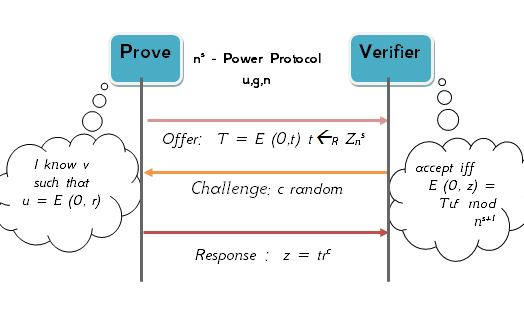
\includegraphics[scale=0.8]{../../Thesis/Pictures/Ch2/ns-power.jpg} 
\caption{$n^s$ Power Protocol - Proof of Knowledge of Randomness}
\end{figure}
\end{frame}

\begin{frame}{Convert to WID proof}
\begin{figure}[htbp]
\centering
\includegraphics[scale=0.3]{../../Thesis/Pictures/Ch4/nswid.jpg} 
\caption{Witness indistinguishable proof of $n^s$ power \cite{Damgard2003}}
\label{fig:nswid}
\end{figure}
Completeness: $E(0,z)=z^{n^s}=t^{n^s} r^{c^{n^s}} = Tr^{n^{s^c}}=TE(0,r)^c=Tu^c$.
\end{frame}

\begin{frame}{Multiple candidates with super ballot}
\begin{itemize}
\item $C$ parallel yes no votes${v_{ij}}_{i=1,j=1}^{N,C}$
\item Proof of validity: $E(v_{ij},r_{ij})$ is   $n^s$ power
\item Proof that exactly $c$ candidates have been voted
\begin{itemize}
\item Release product of randomness $\prod_{i=1}^C r_{ij}$
\item Calculate product of voter votes $V=\prod_{i=1}^C  E(v_{ij},r_{ij})$
\item Prove that $\frac{V}{(1+n)^c}$ is  $n^s$ power
\end{itemize}
\end{itemize}
\end{frame}


\begin{frame}[allowframebreaks]{Baudron counters}
\begin{itemize}
\item Vote for candidate $c$ - Encrypt $D^c$
\item $\sum_{j=0}^{C-1} a_j D^j < n^s \rightarrow C logN < s logn$
\item Prove vote validity: The vote indeed encrypts $D^c$ where $c \in \{0,...,C-1\}  \Leftrightarrow c < C$

\begin{block}{Strategy}
\begin{itemize}
\item Commit to all l bits of the witness
\item Prove that each commitment corresponds to $0,1$
\item Prove that the commitments do not leave out any bits
\end{itemize}

\textbf{Conclusion}: Since l commitments are used the witness $\in [0,2^{l+1}-1]$
\textbf{Complexity}: $O(l)$

\end{block}

\framebreak 
\textbf{Helper:} A protocol to prove that encryptions $e_a,e_b,e_c$ correspond to plaintext $a,b,c$ such that $ab = c \md{n^s}$
 
\begin{figure}[htbp]
\includegraphics[scale=0.3]{../../Thesis/Pictures/Ch4/nsprod.jpg} 
\caption{Proof of Paillier encrypted product \cite{Damgard2003}}
\end{figure}

\framebreak

\item \textbf{Application Case 1:} The number of candidates $C$  is a power of 2 $C=2^{l+1}$
All binary numbers with $l+1$ bits are valid candidates, hence the strategy applies
\begin{itemize}
\item Convert the candidate index to its binary representation
\item $c=b_02^0+b_12^1+\cdots+b_l2^l$ where $b_j \in {0,1}$. Then $D^c = D^{{2^0}^{b_0}}D^{{2^1}^{b_1}} \cdots D^{{2^l}^{b_l}}$ 
\item $D^c$ is a product of powers of two or ones. 
\item The voter encrypts each product term providing encryptions $e_0 = D^{{2^0}^b_0}, e_1 = D^{{2^1}^b_1}, \cdots, e_l=D^{{2^l}^b_l}$
\item Use a WID protocol to prove that $\frac{e_i}{(1+n)^1}$ or $\frac{e_i}{(1+n)^{D^{2^i}}}$ is an $n^s$ power 
\item Calculates the partial products $E_i = \prod_{x=1}^i D^{{2^x}^b_x}$ such that $E_l = D^c$
\item Use the product proof with $a=E_{i-1}, b=e_i, c=E_i$ 
\end{itemize}

\framebreak

\item \textbf{Application Case 2:} The number of candidates $C$ is not a power of 2
Some binary numbers with $l+1$ bits are valid candidates (the ones less than $C$)
\begin{itemize}
\item Follow the same 3 steps as case 1
\item Define $\beta_i = (D^{2^i} - 1)^{-1}  \md{n^s}$
\item Compute ${e'}_i = \frac{e_i}{(1+n)}^{\beta_i} \md{n^2} = Enc(b_i)$
\item $C=(B_l \cdots B_0)_2$
\item $c < C \Leftrightarrow \exists i>0: B_i = 1 \text{ and } b_i = 0  \text{ and } \forall j>i: B_j = b_j $ 
\item Need to prove equality of $j$ indices and inequality of $i$ 
\item $B_i = b_i \Leftrightarrow z_i = \frac{(2B_i-1)(2b_i-1)+1}{2} = 1$
\item $Z_i = z_l \cdots z_{i+1}B_i(b_i-1) = 1 \Leftrightarrow c < C$
\item Use the product proof with $a=Z_{i+1}, b=z_i, c=Z_i$ 
\item Use WID of $n^s$ power protocol to show that $\exists i: Z_i=1$
\end{itemize}
\end{itemize}
\end{frame}


\begin{frame}[allowframebreaks]{References}
\begin{small}
\bibliographystyle{alpha}
\bibliography{homo}
\nocite{*}
\end{small}

\end{frame}
\end{document}
